\documentclass{article}
\usepackage{tikz}

\begin{document}
\title{Positive Cosine Function}
\date{}
\maketitle

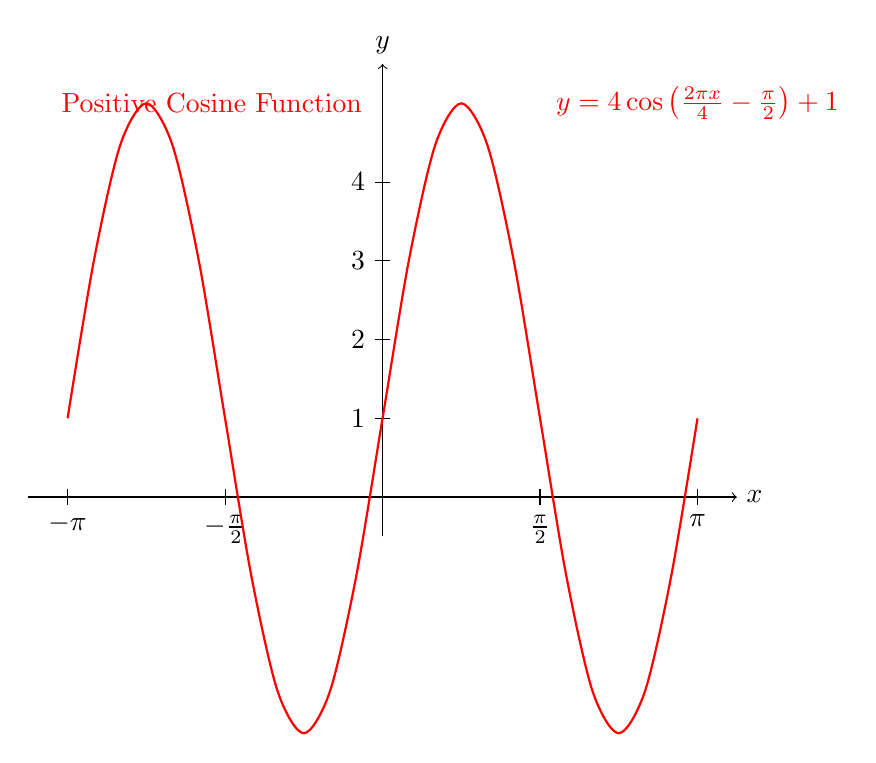
\begin{tikzpicture}
  \draw[->] (-4.5,0) -- (4.5,0) node[right] {$x$};
  \draw[->] (0,-0.5) -- (0,5.5) node[above] {$y$};
  \foreach \x/\xtext in {-4/{-\pi}, -2/{-\frac{\pi}{2}}, 2/{\frac{\pi}{2}}, 4/{\pi}}
    \draw (\x,0.1) -- (\x,-0.1) node[below] {$\xtext$};
  \foreach \y/\ytext in {1/{1}, 2/{2}, 3/{3}, 4/{4}}
    \draw (0.1,\y) -- (-0.1,\y) node[left] {$\ytext$};
  \draw[domain=-4:4, smooth, variable=\x, red, thick] plot ({\x}, {4*cos(360*\x/4 - 90) + 1});
  \node[red, anchor=west] at (-4.2, 5) {Positive Cosine Function};
  \node[red] at (4, 5) {$y = 4 \cos\left(\frac{2\pi x}{4} - \frac{\pi}{2}\right) + 1$};
\end{tikzpicture}

\end{document}
